\documentclass[12pt, a4paper]{article}

\usepackage [utf8]{inputenc}
\usepackage [IL2]{fontenc}
\usepackage [czech]{babel}
\usepackage{graphicx}
\usepackage[numbib]{tocbibind}
\usepackage{hyperref}
\graphicspath{{d:/yyy/}}
\newcommand{\Break}{\State \textbf{break} }

\title{
\includegraphics[width=10cm]{FAV_cmyk}

{\huge Semestrální práce z KIV/TI}

\vspace{0.5cm}
{\LARGE Logické řízení - sanitace nádrží}
\vspace{1cm} 

\Large Lukáš Runt (A20B0226P), Miroslav Vdoviak (A20B....)
\vspace{0.5cm} 

\large \itshape lrunt@students.zcu.cz, lrunt@students.zcu.cz
}
\date{\vspace{6cm} \today}

\begin{document}

\begin{titlepage}
\clearpage\maketitle
\thispagestyle{empty}
\end{titlepage}
\tableofcontents \newpage

\section{Zadání}

\section{Analýza úlohy}

\section{Automatový model}

\subsection{Stavy}
STAV 0 - Systém není v činnosti \newline 
STAV 1 - Tank A se napouští lihem \newline 
STAV 2 - Tanku A se přečerpává čerpadlem \newline 
STAV 3 - Tank A se plní vodou \newline 
STAV 4 - Tank A se proplachuje dokud není ph v normálu \newline 
STAV 5 - Tank A se vypouští \newline 
STAV 6 - Tank B se napouští lihem \newline 
STAV 7 - Tanku B se přečerpává čerpadlem \newline 
STAV 8 - Tank B se plní vodou \newline 
STAV 9 - Tank B se proplachuje dokud není ph v normálu \newline 
STAV 10 - Tank B se vypouští 

\subsection{Snímače}
LA011 - Hladina dosahuje maxima tanku A \newline 
LA010 - Hladina nedosahuje maxima tanku A \newline 
LA021 - Hladina dosahuje minima tanku A \newline 
LA020 - Hladina nedosahuje minima tanku A \newline 
LA031 - Hladina dosahuje maxima tanku B \newline
LA030 - Hladina nedosahuje maxima tanku B \newline 
LA041 - Hladina nedosahuje minima tanku B \newline 
LA040 - Hladina dosahuje minima tanku B

\subsection{Řídící signály}
P0 - Čerpadlo vyplé \newline 
P1 - Čerpadlo zaplé \newline 
Vi0 - Ventil i zavřen \newline 
Vi1 - Ventil i otevřen \newline 
Q0 - Ph nad požadovanou mezí \newline 
Q1 - Ph pod požadovanou mezí 

\subsection{Řízení operátora}
A - Sanitace tanku A \newline 
B - Sanitace tanku B \newline 
Z - Žárovka

\section{Implementace}

\section{Uživatelská příručka}

\subsection{Spuštění programu}
Před spuštěním programu musíme nejprve zkontrolovat, zda se nacházíme ve stejné složce, jako je právě soubor semestralkaTI.jar. Tento program spustíme v příkazové řádce příkazem: \texttt{java -jar semestralkaTI.jar}. Pro spuštění je předpokladem mít nainstalovanou javu verze nejméně 11.

\begin{figure}[h]
\centering 
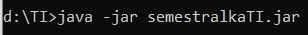
\includegraphics{prikladSpusteni}
\caption{Příklad spuštění}
\end{figure}

Pokud se program podaří spustit zobrazí se model sanitarizace tanků.

\begin{figure}
\centering 
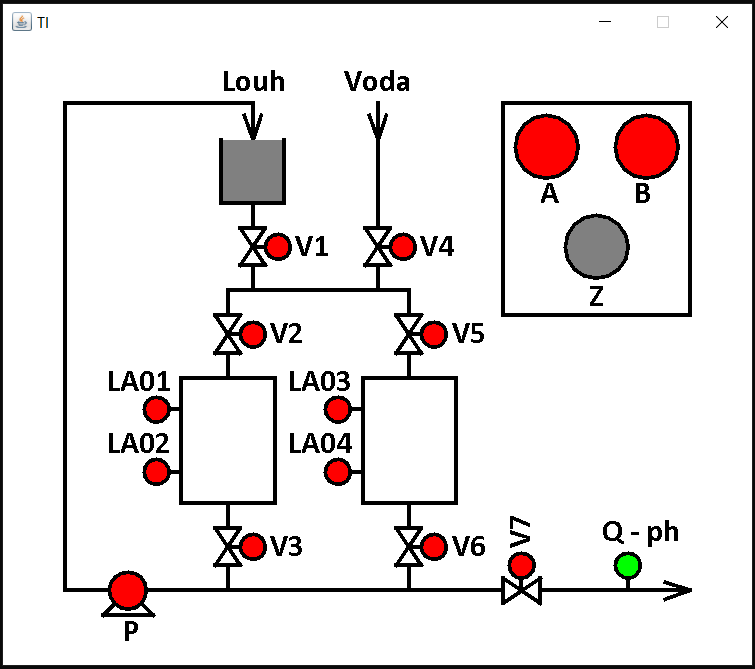
\includegraphics[width=10cm]{vzhledAplikace}
\caption{Vzhled aplikace po spuštění}
\end{figure}

\subsection{Ovládání}
Program se ovládá pomocí klávesnice: \newline 
A - Spuštění sanitarizace tanku A \newline 
B - Spuštění sanitarizace tanku B \newline 
P - Manuální spuštění čerpadla \newline 
1 - Manuální otevření ventilu 1 \newline 
2 - Manuální otevření ventilu 2 \newline 
3 - Manuální otevření ventilu 3 \newline 
4 - Manuální otevření ventilu 4 \newline 
5 - Manuální otevření ventilu 5 \newline 
6 - Manuální otevření ventilu 6 \newline 
7 - Manuální otevření ventilu 7 \newline 


\section{Závěr}
Celkovou práci hodnotím pozitivně, neboť jsem si vyzkoušel napsat konečný automat. Byl to pro mne nepopsatelný zážitek, který mě studijně obohatil a posunul o krok blíže k praktickým aplikacím teoreticky získaných vědomostí. 

\end{document}